\chapter{Appendix}

\section{Repository} \label{app:repository}
All relevant files are also uploaded to a git repository at: \\
\sffamily
codeberg.org/lukaskluge/calibration-and-trajectory-planning-for-a-L-PBF-system
\rmfamily

\section{Code}
\subsection{Calibration MATLAB code} \label{app:calibration-matlab}
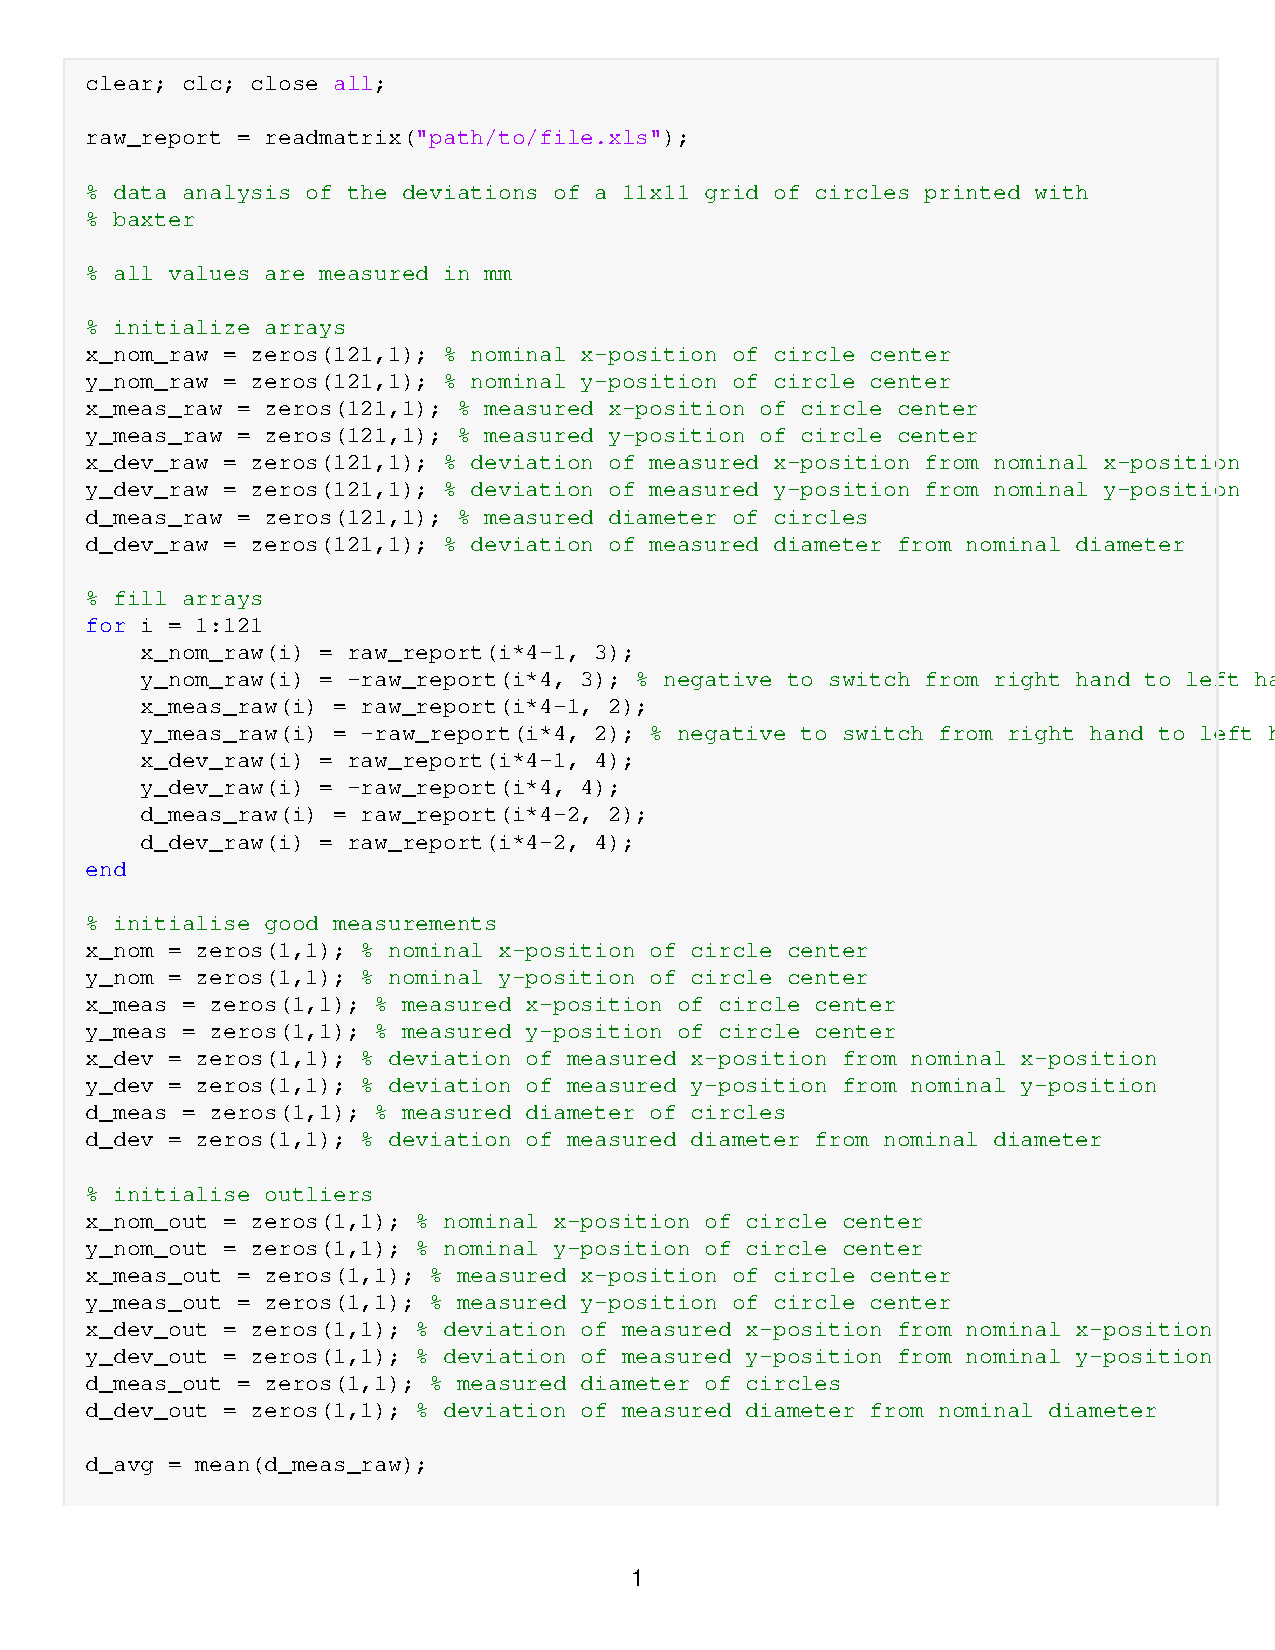
\includepdf[pages=-,pagecommand={},width=\textwidth]{Backmatter/calibration_script_for_report.pdf}
\subsection{Calibration python g-code converter} \label{app:calibration-g-code-python}
\begin{minted}{python}
import sys
import datetime

# usage in terminal:
# $ py g-code calibration.py "filename.g" 0.1 1.09 0.02 -0.3 1.06 -0.05
# (order of the calibration coefficients: qx00 qx10 qx01 qy00 qy10 qy01
# The q00's can be set to zero to keep centre position

# define calibration function (inverse fit)
def calibrate(x, y, qx00, qx10, qx01, qy00, qy10, qy01):
    # Takes as input the desired physical x,y coords plus regression params
    # and gives as output the corresponding corrected g-code x,y vals.
    # The expression stems from the "data-analysis" matlab script
    calX = -(qy00*qx01 - qx00*qy10 + qy10*x - qx01*y)/(qx01*qy01 - qx10*qy10)
    calY = -(qx00*qy01 - qy00*qx10 + qx10*y - qy01*x)/(qy01*qx01 - qy10*qx10)

    return calX, calY

# read inputs
rawFileName = sys.argv[1]
qx00 = sys.argv[2]
qx10 = sys.argv[3]
qx01 = sys.argv[4]
qy00 = sys.argv[5]
qy10 = sys.argv[6]
qy01 = sys.argv[7]

# only creates file if not existing
calibratedFile = open(rawFileName[:-2] + "-calibrated.g", 'x') 

with open(rawFileName, 'r') as rawFile:

    firstEmptyLineFlag = True
    for line in rawFile:
        command = line.split()

        # everything else than G1 commands is just copied
        if len(command) == 0:
            if firstEmptyLineFlag: 
                calibratedFile.write(";Calibrated: " +
                        datetime.datetime.now().isoformat() + "\n")
                firstEmptyLineFlag = False
            calibratedFile.write(line)

        elif command[0] != 'G1':
            calibratedFile.write(line)

        else:
            newLine = 'G1 ' # initiate line for new file.

            i = 1

            #Copy everything before first coordinate
            while i < len(command) and command[i][0] != "X":
                newLine += " " + command[i] 
                i += 1

            # convert coords and write
            if i < len(command): #check if we reached eol already (there are no coords)
                inputX = float(command[i][1:])
                inputY = float(command[i + 1][1:])
                calX, calY = calibrate(inputX, inputY, qx00, qx10, qx01, qy00, qy10, qy01)
                newLine += "X" + str(round(calX, 4)) + " "
                newLine += "Y" + str(round(calY, 4))
            i += 2 # jump to after coords

            # copy everything after coords
            for word in command[i:]:
                newLine += " " + word

            # write to file
            calibratedFile.write(newLine + "\n")

calibratedFile.close()

\end{minted}

\subsection{Fifth order trajectory planning} \label{app:quintic-planning-python}
\begin{minted}{python}
# author: Lukas Kluge, 2022-05-05

import math

def quinticTrajectory(psx0, psy0, psx1, psy1, nsx0, nsy0, nsx1, nsy1,
        pvNorm, nvNorm, cpAvgV, mls, minT, maxPos, maxSpeed):
    #
    # Given information about two melt trajectories, this function
    # calculates a quintic move trajectory that connects them smoothly
    #
    # inputs:
    # psx0 = start x-coord of previous line segment [mm]
    # psy0 = start y-coord of previous line segment [mm]
    #
    # psx1 = end x-coord of previous line segment [mm]
    # psy1 = end y-coord of previous line segment [mm]
    #
    # nsx0 = start x-coord of next line segment [mm]
    # nsy0 = start y-coord of next line segment [mm]
    #
    # nsx1 = end x-coord of next line segment [mm]
    # nsy1 = end y-coord of next line segment [mm]
    #
    # pvNorm = speed (norm of velocity) of previous line
    # nvNorm = speed of next line
    #
    # cpAvgV = desired absolute average velocity of move trajectory [mm/s]
    #
    # mls = max. no. line segments of move trajectory (depends on GLAMS buffer size)
    # minT = min. duration of each line segment [s] (depends on scanner read speed)
    # 
    # maxPos = max. distance the trajectory can deviate from the center of field
    # maxSpeed = max. absolute velocity of the trajectory
    #
    # outputs:
    # array of [x, y, speed] (units [mm, mm, mm/s]) ready for g-code
    #
    # if you don't like short var names use find/replace to change them

    t1 = endTime(psx1, psy1, nsx0, nsy0, cpAvgV)
    beta = quinticPolynomialCoeffs(psx0, psy0, psx1, psy1,
            nsx0, nsy0, nsx1, nsy1, pvNorm, nvNorm, t1)
    t = discreteTime(t1, mls, minT)
    points = len(t)
    sx = [0]*points
    sy = [0]*points
    for i in range(points):
        sx[i] = quinticPolynomial(t[i], beta[0][0], beta[0][1], beta[0][2],
                beta[0][3], beta[0][4], beta[0][5])
        sy[i] = quinticPolynomial(t[i], beta[1][0], beta[1][1], beta[1][2],
                beta[1][3], beta[1][4], beta[1][5])

    limitPosition(points, t, sx, sy, maxPos)
    sNorm = findDistances(points, sx, sy)
    vNorm = findSpeeds(points, t, sNorm)
    limitSpeeds(points, vNorm, t, sNorm, maxSpeed)

    return [sx[1:], sy[1:], vNorm]

def endTime(psx1, psy1, nsx0, nsy0, cpAvgV):
    # The trajectory is assumed to start at t=0.
    # This functions calculates at what time it should end
    cpsNorm = math.sqrt((nsx0-psx1)**2 + (nsy0-psy1)**2)
    return cpsNorm/cpAvgV

def quinticPolynomialCoeffs(psx0, psy0, psx1, psy1, nsx0, nsy0, nsx1, nsy1,
        pvNorm, nvNorm, t1):
    # This calculates the coefficients of the polynomials describing the trajectory
    # TODO refactor into two functions: find boundary conditions and find coeffs

    psNorm = math.sqrt((psx1-psx0)**2 + (psy1-psy0)**2) 
    pvx = (psx1-psx0)/psNorm*pvNorm # prev vel in x-direction
    pvy = (psy1-psy0)/psNorm*pvNorm # prev vel in y-direction

    nsNorm = math.sqrt((nsx1-nsx0)**2 + (nsy1-nsy0)**2)
    nvx = (nsx1-nsx0)/nsNorm*nvNorm # nrev vel in x-direction
    nvy = (nsy1-nsy0)/nsNorm*nvNorm # nrev vel in y-direction

    # x polynomial coefficients
    betax0 = psx1
    betax1 = pvx
    betax2 = 0
    betax3 = -(10*psx1 - 10*nsx0 + t1*(6*pvx + 4*nvx))/(t1**3)
    betax4 = (15*psx1 - 15*nsx0 + t1*(8*pvx + 7*nvx))/(t1**4)
    betax5 = -(6*psx1 - 6*nsx0 + t1*(3*pvx + 3*nvx))/(t1**5)

    # y polynomial coefficients
    betay0 = psy1
    betay1 = pvy
    betay2 = 0
    betay3 = -(10*psy1 - 10*nsy0 + t1*(6*pvy + 4*nvy))/(t1**3)
    betay4 = (15*psy1 - 15*nsy0 + t1*(8*pvy + 7*nvy))/(t1**4)
    betay5 = -(6*psy1 - 6*nsy0 + t1*(3*pvy + 3*nvy))/(t1**5)

    return [[betax0, betax1, betax2, betax3, betax4, betax5],
            [betay0, betay1, betay2, betay3, betay4, betay5]]

def discreteTime(t1, mls, minT):
    if (t1/minT <= mls):
        ls = math.floor(t1/minT)
        nomT = t1/ls # nominal T (actual dt might differ after limit correction)
        tDiscrete = [0]*(ls+1) # initialise
        for i in range(ls+1):
            tDiscrete[i] = nomT*i
    else:
        nomT = t1/mls # nominal T (actual dt might differ after limit correction)
        tDiscrete = [0]*(mls+1) # initialise
        for i in range(mls+1):
            tDiscrete[i] = nomT*i
    return tDiscrete

def quinticPolynomial(t, beta0, beta1, beta2, beta3, beta4, beta5):
    return beta0 + beta1*t + beta2*t**2 + beta3*t**3 + beta4*t**4 + beta5*t**5

def limitPosition(points, t, sx, sy, maxPos):
    for i in range(points):
        if sx[i] > maxPos:
            sx[i] = maxPos
        elif sx[i] < -maxPos:
            sx[i] = -maxPos
        if sy[i] > maxPos:
            sy[i] = maxPos
        elif sy[i] < -maxPos:
            sy[i] = -maxPos
    return [t, sx, sy]

def findDistances(points, sx, sy):
    sNorm = [0]*(points - 1)
    for i in range(points - 1):
        sNorm[i] = math.sqrt((sx[i+1]-sx[i])**2 + (sy[i+1]-sy[i])**2)
    return sNorm

def findSpeeds(points, t, sNorm):
    vNorm = [0]*(points - 1)
    for i in range(points - 1):
        T = t[i+1] - t[i]
        vNorm[i] = sNorm[i]/T
    return vNorm

def limitSpeeds(points, vNorm, t, sNorm, maxSpeed):
    Tnom = t[1] # nominal time interval (before speed limit)
    for i in range(points-1):
        if vNorm[i] > maxSpeed:
            vNorm[i] = maxSpeed
            t[i+1] = t[i] + sNorm[i]/maxSpeed
            for j in range((i+1),points-1):
                t[j] = t[j] + (sNorm[j]/maxSpeed - Tnom)
    return vNorm

\end{minted}
\subsection{Modified third order trajectory planning} \label{app:cubic-planning-python}
\begin{minted}{python}
# author: Lukas Kluge, 2022-05-05

import math

def cubicTrajectory(psx1, psy1, nsx0, nsy0, nsx1, nsy1,
        nvNorm, mls, minT, maxPos, maxSpeed):
    #
    # Given information about two melt trajectories, this function
    # calculates a cubic move trajectory that starts at max velocity
    #
    #
    # inputs:
    #
    # psx1 = end x-coord of previous line segment [mm]
    # psy1 = end y-coord of previous line segment [mm]
    #
    # nsx0 = start x-coord of next line segment [mm]
    # nsy0 = start y-coord of next line segment [mm]
    #
    # nsx1 = end x-coord of next line segment [mm]
    # nsy1 = end y-coord of next line segment [mm]
    #
    # nvNorm = speed (norm of velocity) of next line
    #
    # mls = max. no. line segments of move trajectory (depends on GLAMS buffer size)
    # minT = min. duration of each line segment [s] (depends on scanner read speed)
    # 
    # maxPos = max. distance the trajectory can deviate from the center of field
    # maxSpeed = max. absolute velocity of the trajectory.
    # Should be at least three times higher than nvNorm (see t1x, t1y)
    #
    # outputs:
    # array of [x, y, speed] (units [mm, mm, mm/s]) ready for g-code
    #
    # if you don't like short var names use find/replace to change them

    t1 = endTime(psx1, psy1, nsx0, nsy0, nsx1, nsy1,
            nvNorm, maxSpeed)
    beta = cubicPolynomialCoeffs(psx1, psy1,
            nsx0, nsy0, nsx1, nsy1, nvNorm, t1)
    t = discreteTime(t1, mls, minT)
    points = len(t)
    sx = [0]*points
    sy = [0]*points
    for i in range(points):
        sx[i] = cubicPolynomial(t[i], beta[0][0], beta[0][1], beta[0][2],
                beta[0][3])
        sy[i] = cubicPolynomial(t[i], beta[1][0], beta[1][1], beta[1][2],
                beta[1][3])

    limitPosition(points, t, sx, sy, maxPos)
    sNorm = findDistances(points, sx, sy)
    vNorm = findSpeeds(points, t, sNorm)

    return [sx[1:], sy[1:], vNorm]

def endTime(psx1, psy1, nsx0, nsy0, nsx1, nsy1,
        nvNorm, maxSpeed):
    # The trajectory is assumed to start at t=0.
    # This functions calculates at what time it should end

    # find maxSpeed in each direction, taking into account
    # norm max speed and sign to get a positive t1
    maxSpeedx = 0.7071*math.copysign(maxSpeed, nsx0-psx1)
    maxSpeedy = 0.7071*math.copysign(maxSpeed, nsy0-psy1)
    
    nsNorm = math.sqrt((nsx1-nsx0)**2 + (nsy1-nsy0)**2)
    nvx = (nsx1-nsx0)/nsNorm*nvNorm # next vel in x-direction
    nvy = (nsy1-nsy0)/nsNorm*nvNorm # next vel in y-direction

    t1x = (3*nsx0-3*psx1)/(2*nvx+maxSpeedx)
    t1y = (3*nsy0-3*psy1)/(2*nvy+maxSpeedy)

    return t1x if (t1x>t1y) else t1y

def cubicPolynomialCoeffs(psx1, psy1, nsx0, nsy0, nsx1, nsy1,
        nvNorm, t1):
    # This calculates the coefficients of the polynomials describing the trajectory
    # TODO refactor into two functions: find boundary conditions and find coeffs

    nsNorm = math.sqrt((nsx1-nsx0)**2 + (nsy1-nsy0)**2)
    nvx = (nsx1-nsx0)/nsNorm*nvNorm # nrev vel in x-direction
    nvy = (nsy1-nsy0)/nsNorm*nvNorm # nrev vel in y-direction

    # x polynomial coefficients
    betax0 = psx1
    betax1 = -(3*psx1 - 3*nsx0 + 2*t1*nvx)/t1
    betax2 = (3*(psx1 - nsx0 + t1*nvx))/t1**2
    betax3 = -(psx1 - nsx0 + t1*nvx)/t1**3

    # y polynomial coefficients
    betay0 = psy1
    betay1 = -(3*psy1 - 3*nsy0 + 2*t1*nvy)/t1
    betay2 = (3*(psy1 - nsy0 + t1*nvy))/t1**2
    betay3 = -(psy1 - nsy0 + t1*nvy)/t1**3

    return [[betax0, betax1, betax2, betax3],
            [betay0, betay1, betay2, betay3]]

def discreteTime(t1, mls, minT):
    if (t1/minT <= mls):
        ls = math.floor(t1/minT)
        nomT = t1/ls # nominal T (actual dt might differ after limit correction)
        tDiscrete = [0]*(ls+1) # initialise
        for i in range(ls+1):
            tDiscrete[i] = nomT*i
    else:
        nomT = t1/mls # nominal T (actual dt might differ after limit correction)
        tDiscrete = [0]*(mls+1) # initialise
        for i in range(mls+1):
            tDiscrete[i] = nomT*i
    return tDiscrete

def cubicPolynomial(t, beta0, beta1, beta2, beta3):
    return beta0 + beta1*t + beta2*t**2 + beta3*t**3

def limitPosition(points, t, sx, sy, maxPos):
    for i in range(points):
        if sx[i] > maxPos:
            sx[i] = maxPos
        elif sx[i] < -maxPos:
            sx[i] = -maxPos
        if sy[i] > maxPos:
            sy[i] = maxPos
        elif sy[i] < -maxPos:
            sy[i] = -maxPos
    return [t, sx, sy]

def findDistances(points, sx, sy):
    sNorm = [0]*(points - 1)
    for i in range(points - 1):
        sNorm[i] = math.sqrt((sx[i+1]-sx[i])**2 + (sy[i+1]-sy[i])**2)
    return sNorm

def findSpeeds(points, t, sNorm):
    vNorm = [0]*(points - 1)
    for i in range(points - 1):
        T = t[i+1] - t[i]
        vNorm[i] = sNorm[i]/T
    return vNorm
\end{minted}
\subsection{Trajectory planning python g-code converter} \label{app:traj-g-code}
\begin{minted}{python}
# g-code-trajectory-insert

# usage in terminal: 
# $ py g-code-trajectory-insert.py "filename.g" 57.5 1000 600 63 0.00002 3
# order of arguments: maxPos maxSpeed cpAvgV mls minT style

import sys
import datetime

import quinticTrajectory as q
import cubicTrajectory as c

rawFileName = sys.argv[1]
maxPos = float(sys.argv[2])
maxSpeed = float(sys.argv[3])
cpAvgV = float(sys.argv[4]) # irrelevant for cubic
mls = int(sys.argv[5]) # GLAMS g-code buffer size
minT = float(sys.argv[6]) # less than read speed of scanner
style = int(sys.argv[7]) # 3 or 5 for cubic or quintic trajectories

def isMeltLine(line):
    coords = line.find("X")
    density = line.find("D")
    return (coords > -1) and (density > -1) and int(line[density+1]) > 0

def isMoveLine(line):
    coords = line.find("X")
    density = line.find("D")
    return (coords > -1) and ((density == -1) or int(line[density+1]) == 0)

def isSpeedChange(command):
    speed = -1
    for x in command:
        if x[0] == 'F':
            speed = float(x[1:])
    return speed

def findCoords(command):
    i = 0
    while i < len(command) and command[i][0] != "X":
        i += 1

    inputX = float(command[i][1:])
    inputY = float(command[i + 1][1:])
    return [inputX, inputY]

# create file with trajectories if not existing
fileWithTrajectories = open(rawFileName[:-2] + "-with-" + str(style) +
        "trajectories.g", 'x')

# read original file and fill new file accordingly
with open(rawFileName, 'r') as rawFile:
    firstEmptyLineFlag = True # checks where to add "trajectories added" note
    sa = [0, 0] # init most recent position [x [mm], y [mm]]
    sb = [-1, 0] # init second most recent position
    sc = [0, 0] # init third most recent position
    sd = [0, 0] # init fourth most recent position 
    pba = [0, True] # init path from sb to sa [speed, laser on?]
    pcb = [0, False] # init path from sc to sb
    pdc = [0, False] # init path from sd to sc
    cache = [sa, pba, sb, pcb, sc, pdc, sd] # array of previous movements
    currentSpeed = 0 # speed is set asynchroniously in the g-code, thus need var

    for line in rawFile:
        command = line.split() # divide into components

        if len(command) == 0:
            # add metadata about added trajectories,
            if firstEmptyLineFlag:
                fileWithTrajectories.write(";Trajectories added: " +
                        datetime.datetime.now().isoformat() + "\n")
                fileWithTrajectories.write(";Max position: " +
                        '%.5f' % maxPos + "\n")
                fileWithTrajectories.write(";Max speed: " +
                        '%.5f' % maxSpeed + "\n")
                fileWithTrajectories.write(";Min T (time for one movement): " +
                        '%.5f' % minT + "\n")
                fileWithTrajectories.write(";average speed of move trajectories: " +
                        '%.5f' % cpAvgV + "\n")
                fileWithTrajectories.write(";Max line segments: " +
                        '%.5f' % mls + "\n")
                fileWithTrajectories.write(";polynomial type (3rd or 5th order): " +
                        '%.5f' % style + "\n")

                firstEmptyLineFlag = False
            # copy (empty) line to output
            fileWithTrajectories.write(line)

        # copy lines that are not about movement directly to output
        elif command[0] != 'G1':
            fileWithTrajectories.write(line)

        # check if line moves the off laser and store info if it does
        elif isMoveLine(line):
            sd = sc
            sc = sb
            sb = sa
            sa = findCoords(command)

            pdc = pcb
            pcb = pba
            pba = [currentSpeed, False]

            if not pcb[1]:
                fileWithTrajectories.write(line) # TODO write previous line instead

        
        # check if line moves the on laser and print the appropriate
        # move trajectory to lead up to and including that line.
        elif isMeltLine(line):
            # make room for new position
            sd = sc
            sc = sb
            sb = sa
            sa = findCoords(command) # add newest position

            # make room for new path
            pdc = pcb
            pcb = pba
            pba = [currentSpeed, True] # add newest path

            if not pcb[1]: # check if previous line was move line 
                if style == 5: # quintic
                    moveTrajectory = q.quinticTrajectory(sd[0], sd[1], sc[0], sc[1],
                            sb[0], sb[1], sa[0], sa[1],
                            pdc[0], pba[0], cpAvgV, mls, minT, maxPos, maxSpeed)
                elif style == 3: # cubic
                    moveTrajectory = c.cubicTrajectory(sc[0], sc[1], sb[0], sb[1],
                            sa[0], sa[1], pba[0], mls, minT, maxPos, maxSpeed)

                # print move trajectory g-code and melt trajectory g-code
                for i in range(len(moveTrajectory[0])):
                    # speed
                    fileWithTrajectories.write(
                            "G1 F" + '%.6f' % moveTrajectory[2][i] + "\n")
                    # position (add D at the end if the laser should be on)
                    fileWithTrajectories.write(
                            "G1 X" + '%.6f' % moveTrajectory[0][i] + " Y" +
                                    '%.6f' % moveTrajectory[1][i] + "\n")
                
                fileWithTrajectories.write("G1 F" + str(pba[0]) + "\n")
                fileWithTrajectories.write(line)

        # other G-commands should there be any,
        # are just copied to output file
        else: 
            if isSpeedChange(command) > -1: 
                currentSpeed = isSpeedChange(command)
            fileWithTrajectories.write(line)

fileWithTrajectories.close()

\end{minted}

\section{Experiment data}
\subsection{Calibration experiment before} \label{app:calibration-data}
\nopagecolor
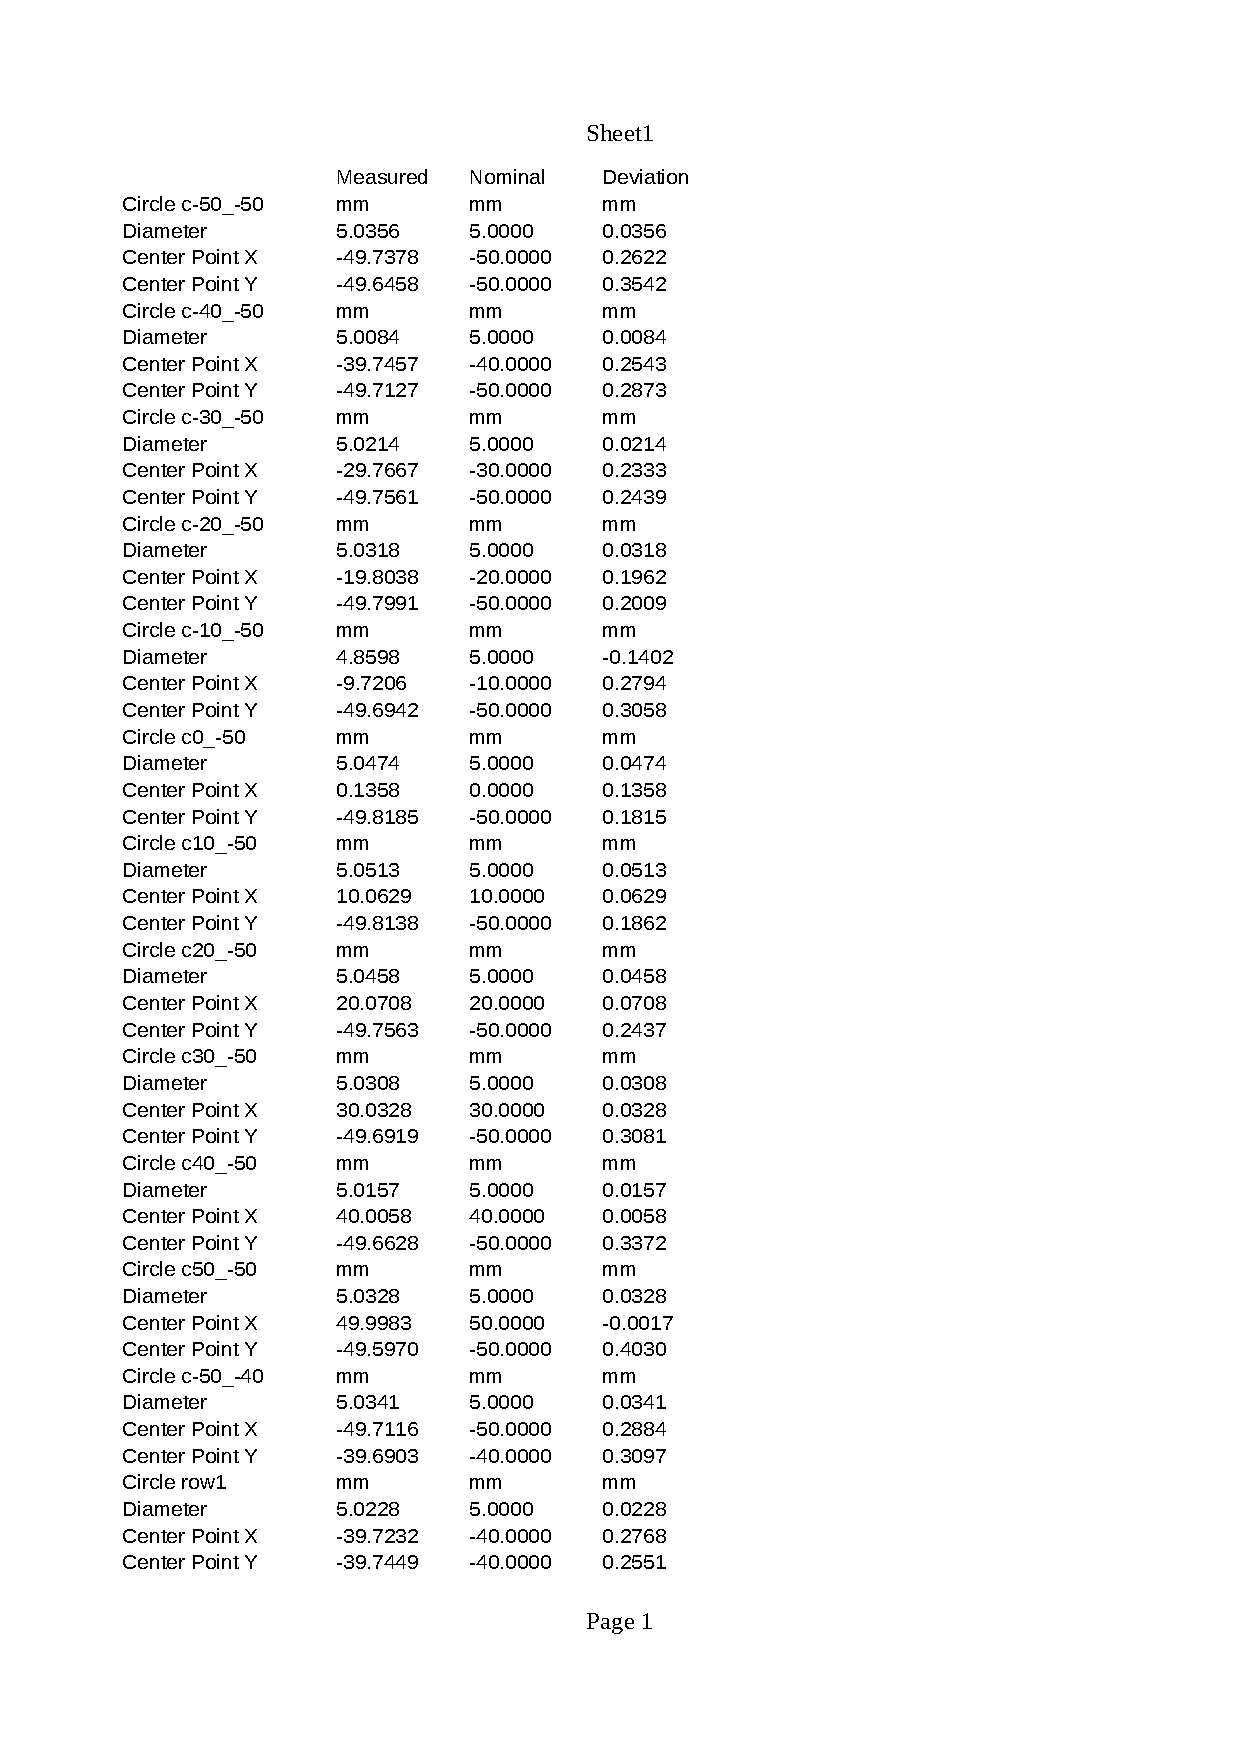
\includepdf[width=1.3\linewidth,pages=-]{Backmatter/calibration-measurement-data.pdf}
%\includepdf[pages=-,width=0.5\textwidth]{Backmatter/2022-05-24-1426.pdf}
\subsection{Calibration experiment after} \label{app:verification-data}
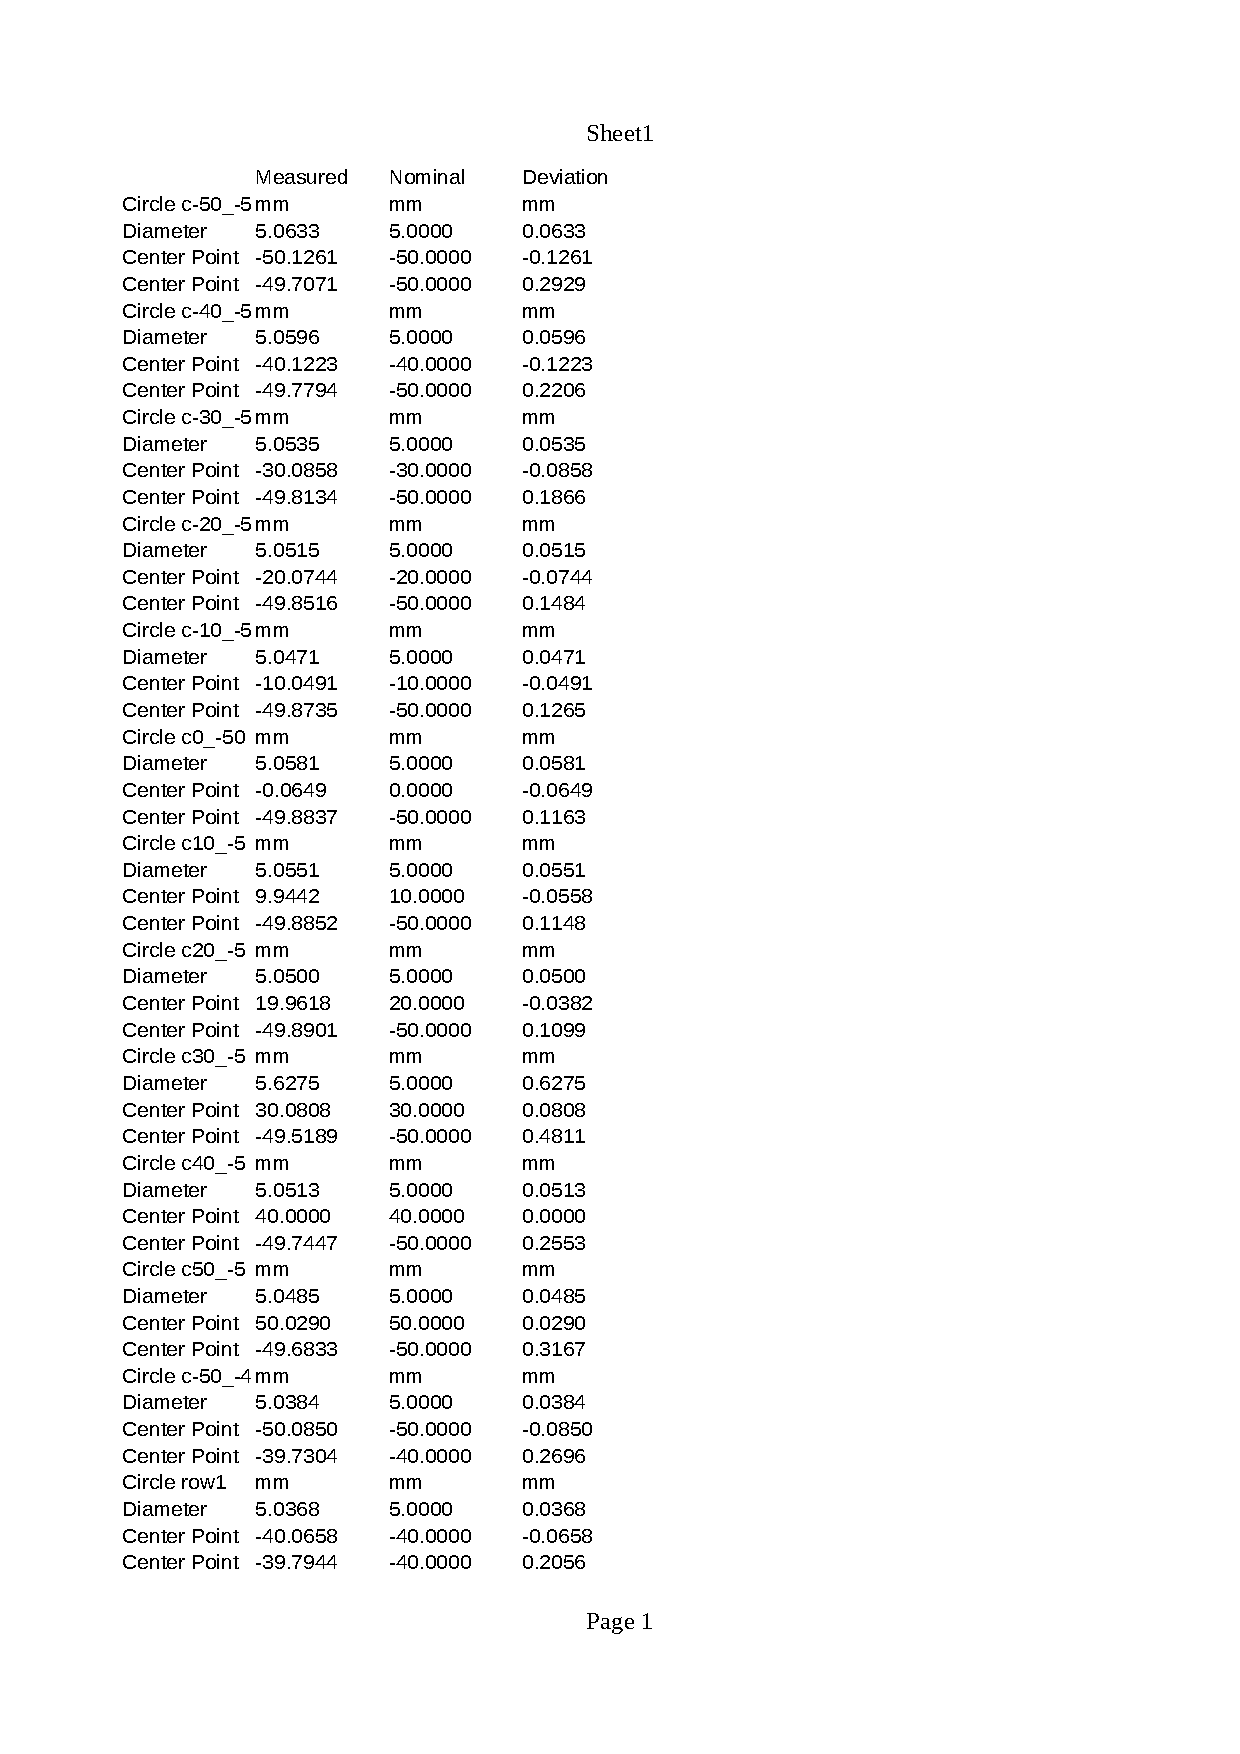
\includepdf[pages=-,pagecommand={},width=1.3\linewidth]{Backmatter/verification-measurements-data.pdf}

